%! Author = crist
%! Date = 25/10/2026

\spacing{1.3}
%----------------------------------------------------------------------------------------
%	UNIDAD 5: LA MATERIA Y LOS SISTEMAS MATERIALES (4.º ESO)
%   Figuras: images/UD5/*.pdf (fuente HTML en images/UD5/html, SVG en images/UD5/svg)
%----------------------------------------------------------------------------------------

% Unidades de presión que se usan en la unidad
\DeclareSIUnit\atm{atm}
\DeclareSIUnit\mmHg{mmHg}

% Mapa conceptual del tema (fuente en images/mapas_conceptuales/html/temas.js)
\begin{figure}[H]
    \centering
    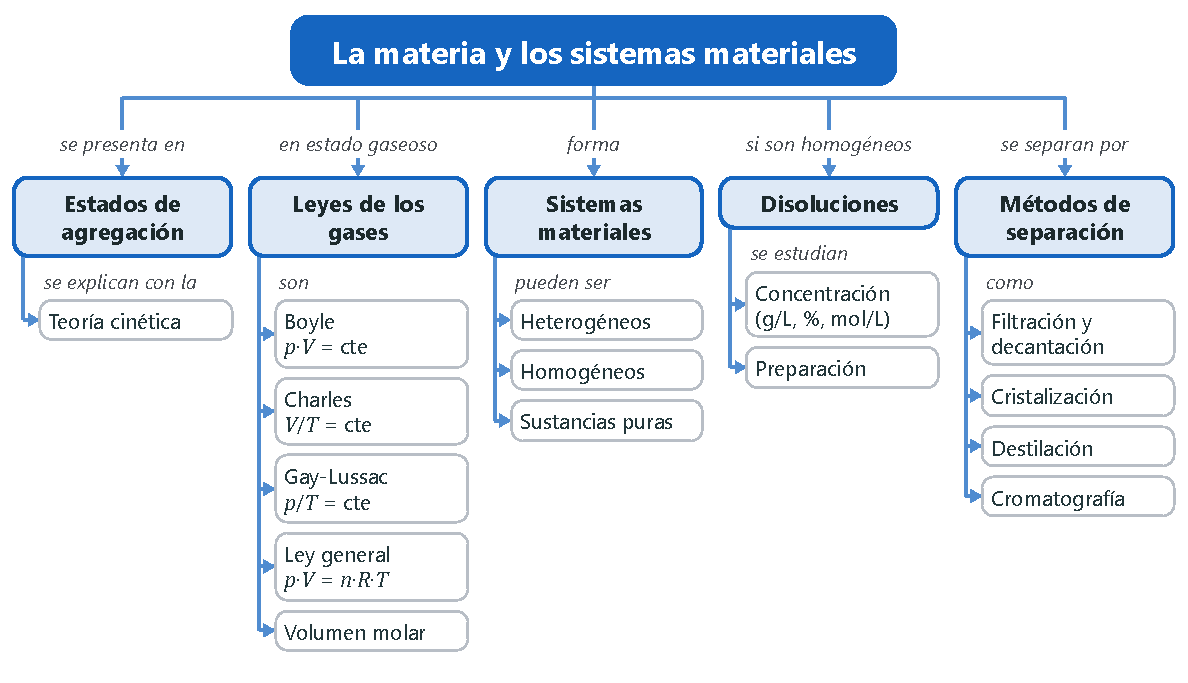
\includegraphics[width=\textwidth]{images/mapas_conceptuales/mapa_UD5}
\end{figure}

%========================================================================================
%\section*{Para empezar: la atmósfera y la capa de ozono}
%\addcontentsline{toc}{section}{Para empezar: la atmósfera y la capa de ozono}
%========================================================================================
%
%La \textbf{atmósfera} es un sistema material gaseoso que contiene los gases imprescindibles para la vida, sobre todo nitrógeno y oxígeno, y en ella tiene lugar el ciclo del agua: evaporación, condensación y precipitación. Aunque el límite científico con el espacio está a unos \qty{104}{\km} de altura, en aviación y astronáutica se toma como frontera la \textbf{línea de Kármán}, a \qty{100}{\km} sobre el nivel del mar.
%
%Entre los 15 y los \qty{50}{\km} de altitud se encuentra la \textbf{capa de ozono}, que reúne el \qty{90}{\percent} del ozono (\ch{O3}) atmosférico y absorbe el \qty{98}{\percent} de la radiación ultravioleta más energética del Sol. Sin ella, esa radiación dañaría a los seres vivos: provoca cáncer de piel, cataratas y otros problemas (figura~\ref{fig:atmosfera_ozono}).
%
%En los años 70 y 80 del siglo pasado se descubrió que el ozono sobre la Antártida estaba disminuyendo. Uno de los principales culpables eran los \textbf{clorofluorocarbonos} (CFC), gases que se usaban en frigoríficos, en la fabricación de espumas y como propelentes de los aerosoles. El agujero cambia de tamaño a lo largo del año y alcanza sus valores mínimos de ozono durante el invierno austral. En 2022 llegó a medir de media unos 23 millones de kilómetros cuadrados, algo menos que el año anterior. Esta mejora se debe, con toda probabilidad, al \textbf{Protocolo de Montreal} (1987), por el que muchos países se comprometieron a dejar de usar los CFC.
%
%\begin{figure}[H]
%    \centering
%    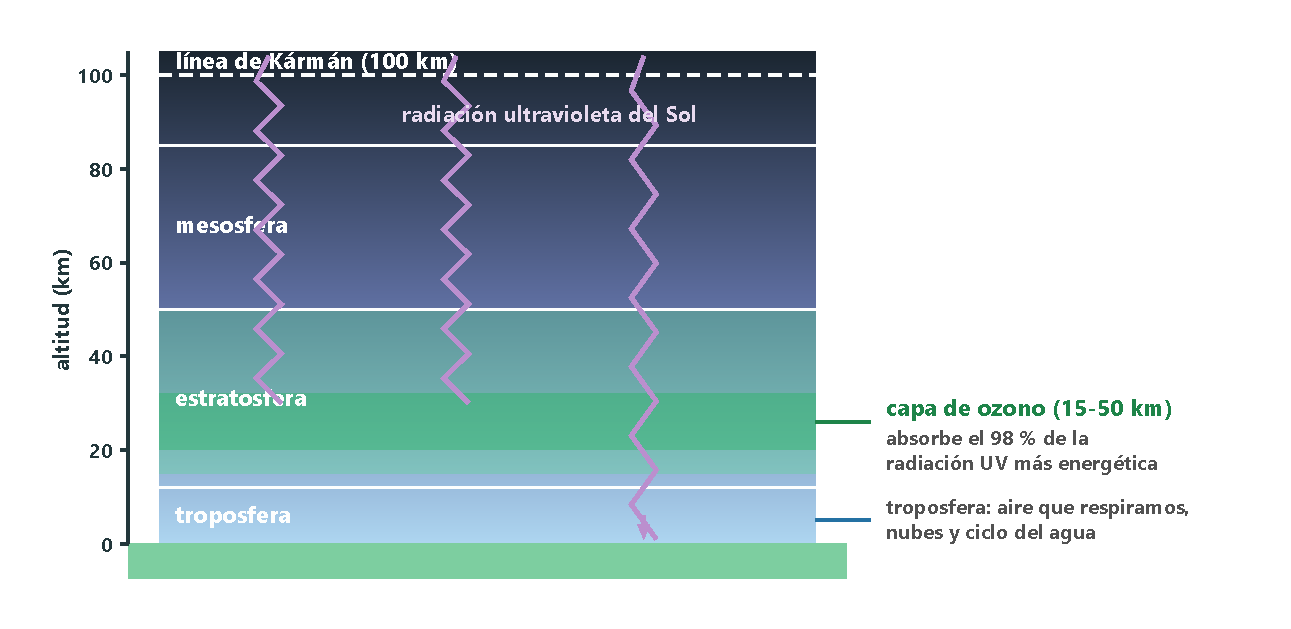
\includegraphics[width=0.85\textwidth]{images/UD5/atmosfera_ozono}
%    \caption{Capas de la atmósfera y situación de la capa de ozono.}
%    \label{fig:atmosfera_ozono}
%\end{figure}
%
%\begin{remark}
%    \textbf{Ozono y Objetivos de Desarrollo Sostenible.} Reducir el agujero de la capa de ozono está relacionado con el \textbf{ODS 3} (\emph{Salud y bienestar}), cuya meta 3.9 pide reducir las muertes y enfermedades causadas por productos químicos peligrosos y por la contaminación del aire, y con el \textbf{ODS 12} (\emph{Producción y consumo responsables}), cuya meta 12.4 busca reducir la liberación de productos químicos a la atmósfera, el agua y el suelo.
%\end{remark}
%
%\begin{exercise}
%    ¿Por qué decimos que la atmósfera es un sistema material gaseoso? ¿Qué papel juega en la existencia de vida en la Tierra?
%    \begin{solu}
%        Porque es una porción de materia formada por \textcolor{red}{gases}. Contiene los gases necesarios para la vida (oxígeno y nitrógeno, principalmente) y en ella se produce el \textcolor{red}{ciclo del agua}: evaporación, condensación y precipitación.
%    \end{solu}
%\end{exercise}
%
%\begin{exercise}
%    ¿Qué es la capa de ozono? ¿A qué altura está y por qué es tan importante para los seres vivos?
%    \begin{solu}
%        Es la zona de la atmósfera, situada entre los \textcolor{red}{15 y los \qty{50}{\km}} de altitud, que contiene el \qty{90}{\percent} del ozono atmosférico. Es importante porque \textcolor{red}{absorbe el \qty{98}{\percent} de la radiación ultravioleta} más energética, que de otro modo produciría cáncer de piel, cataratas y otros daños.
%    \end{solu}
%\end{exercise}
%
%\begin{exercise}
%    ¿Qué sustancias provocaron la aparición del agujero de ozono? ¿En qué época del año es más grande? ¿Por qué fue tan importante el Protocolo de Montreal?
%    \begin{solu}
%        Los \textcolor{red}{clorofluorocarbonos (CFC)}, usados en frigoríficos, espumas y aerosoles. Los valores mínimos de ozono se registran durante el \textcolor{red}{invierno austral} (septiembre y octubre). El Protocolo de Montreal fue un \textcolor{red}{compromiso internacional para dejar de usar los CFC}; gracias a él, el agujero se está reduciendo.
%    \end{solu}
%\end{exercise}
%
%\begin{exercise}
%    Relaciona la reducción del agujero de la capa de ozono con los ODS 3 y 12.
%    \begin{solu}
%        El \textcolor{red}{ODS 3} (meta 3.9) pretende reducir las muertes y enfermedades causadas por productos químicos como los CFC. El \textcolor{red}{ODS 12} (meta 12.4) busca reducir la liberación de productos químicos a la atmósfera.
%    \end{solu}
%\end{exercise}

%========================================================================================
\section{¿Qué es la materia y cómo se presenta?}
%========================================================================================

\begin{definition}[Materia y sustancia]
    La \textbf{materia} es todo aquello que tiene masa y ocupa un volumen. Cada una de las distintas clases de materia es una \textbf{sustancia}.
\end{definition}

La materia se presenta en tres \textbf{estados de agregación}: sólido, líquido y gaseoso. El estado de una sustancia depende de la intensidad de las \textbf{fuerzas de atracción} (o de cohesión) entre sus partículas comparada con su \textbf{movimiento} (vibración o agitación térmica). Recuerda lo que aprendiste sobre el enlace químico en la unidad anterior: el tipo de enlace determina esas fuerzas.

\begin{figure}[H]
    \centering
    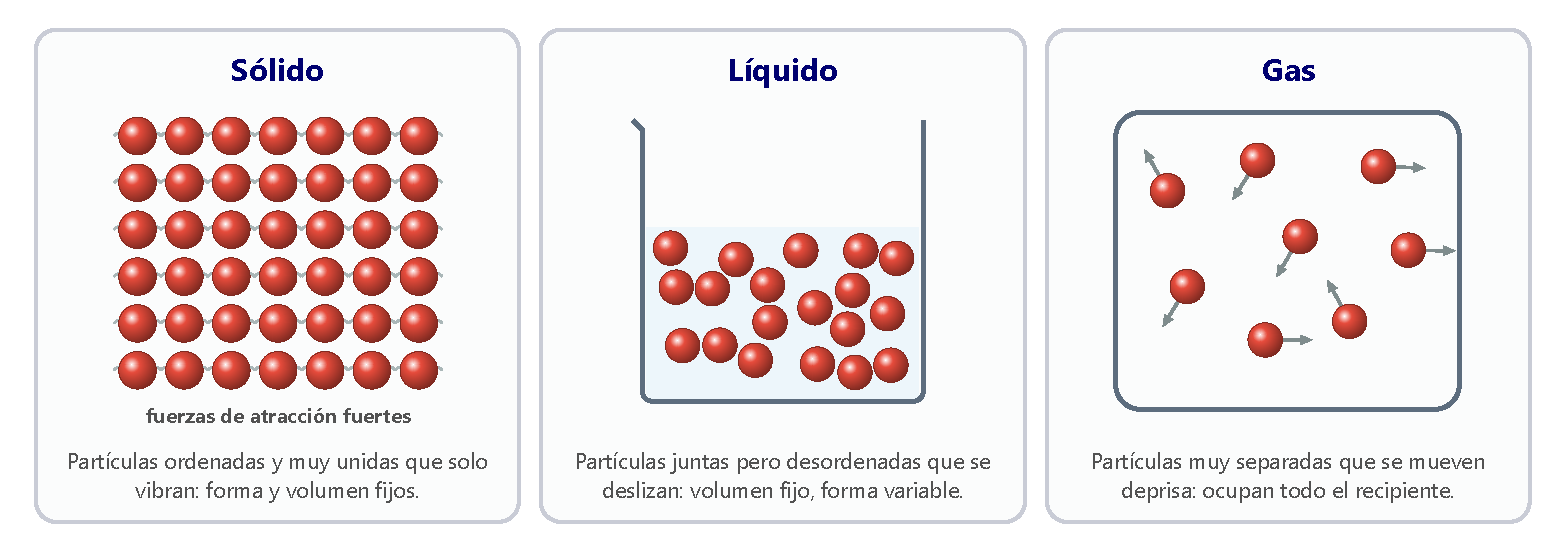
\includegraphics[width=\textwidth]{images/UD5/estados_materia}
    \caption{Modelo de partículas de los tres estados de agregación.}
    \label{fig:estados_materia}
\end{figure}

\begin{itemize}
    \item \textbf{Sólidos.} Las fuerzas de cohesión entre las partículas son mucho más fuertes que su vibración: las partículas ocupan posiciones fijas y el sólido tiene \textbf{forma y volumen propios}. Son sólidos a temperatura ambiente los cristales covalentes (diamante, grafito, \ch{SiO2}), los metales (excepto el mercurio) y los compuestos iónicos como el \ch{NaCl}.
    \item \textbf{Líquidos.} Las fuerzas de cohesión son menores que en los sólidos: las partículas se deslizan unas sobre otras, por eso los líquidos \textbf{fluyen} y se adaptan a la \textbf{forma del recipiente}, aunque su \textbf{volumen no cambia}. El agua (entre 0 y \qty{100}{\celsius}) y el etanol (entre \num{-114} y \qty{78}{\celsius}) son líquidos cuyas moléculas se unen por enlaces de hidrógeno.
    \item \textbf{Gases.} Las fuerzas entre las partículas son muy débiles: se mueven continuamente, de forma desordenada y a gran velocidad, chocando entre sí y con las paredes. Por eso los gases \textbf{ejercen presión}, \textbf{se expanden} hasta ocupar todo el recipiente y \textbf{se pueden comprimir}. Son gases a temperatura ambiente los gases nobles, el \ch{H2}, el \ch{O2}, el \ch{N2}, el \ch{CO2}, el metano o el butano.
\end{itemize}

En los gases, la presión, el volumen y la temperatura están muy relacionados: si cambia una de estas magnitudes, cambian las otras.

\begin{exercise}
    Nombra tres sustancias que sean sólidas, tres líquidas y tres gaseosas a temperatura ambiente. ¿Conoces alguna sustancia que podamos encontrar en la naturaleza en los tres estados?
    \begin{solu}
        Respuesta libre. Sólidos: cloruro de sodio, hierro, diamante. Líquidos: agua, mercurio, etanol. Gases: oxígeno, dióxido de carbono, butano. El \textcolor{red}{agua} se encuentra en la naturaleza como hielo, agua líquida y vapor.
    \end{solu}
\end{exercise}

\begin{exercise}
    Explica, comparando las fuerzas de cohesión con la agitación de las partículas, por qué\ldots
    \begin{enumerate}[label=\alph*)]
        \item un sólido tiene forma y volumen fijos;
        \item un gas tiende a ocupar todo el volumen disponible;
        \item las partículas de un líquido no ocupan posiciones fijas;
        \item un gas ejerce presión sobre las paredes del recipiente;
        \item un líquido fluye y se adapta a la forma del recipiente.
    \end{enumerate}
    \begin{solu}
        a) Las fuerzas de cohesión son \textcolor{red}{mucho mayores} que la vibración de las partículas. b) La agitación de las partículas es \textcolor{red}{mucho mayor} que las fuerzas de cohesión. c) y e) Las fuerzas de cohesión \textcolor{red}{no son tan intensas como en los sólidos}: mantienen las partículas juntas pero les permiten deslizarse. d) Las partículas se mueven muy deprisa y \textcolor{red}{chocan continuamente} contra las paredes.
    \end{solu}
\end{exercise}

\begin{exercise}
    Los gases combustibles más usados son el butano, el propano y el gas natural (metano). En las mismas condiciones, la densidad del aire es \qty{1.3}{\kg\per\cubic\metre}, la del butano \qty{2.6}{\kg\per\cubic\metre}, la del propano \qty{1.9}{\kg\per\cubic\metre} y la del metano \qty{0.7}{\kg\per\cubic\metre}.
    \begin{enumerate}[label=\alph*)]
        \item ¿Dónde se acumula cada gas si hay una fuga?
        \item Busca qué medidas de seguridad se toman en los lugares donde se usan estos gases.
    \end{enumerate}
    \begin{solu}
        a) El butano y el propano son \textcolor{red}{más densos que el aire}: se acumulan \textcolor{red}{cerca del suelo}. El metano es menos denso: \textcolor{red}{sube y se acumula cerca del techo}.
        b) Respuesta libre: rejillas de ventilación a ras de suelo (butano, propano) o en la parte alta (gas natural), detectores de gas, revisiones periódicas de la instalación, no hacer chispas ni encender interruptores si se nota olor a gas\ldots
    \end{solu}
\end{exercise}

\begin{exercise}
    Se coloca un globo desinflado en la boca de un matraz con agua y se añade una pastilla efervescente. Explica lo que le sucede al globo.
    \begin{solu}
        La pastilla desprende un gas (\ch{CO2}). Los gases tienen masa y ocupan un volumen, y su volumen es variable: el gas \textcolor{red}{se expande} y ejerce presión sobre las paredes del globo, que \textcolor{red}{se infla}.
    \end{solu}
\end{exercise}

\begin{exercise}
    ¿Pueden estar dos gases en el mismo recipiente sin mezclarse? Razona tu respuesta.
    \begin{solu}
        \textcolor{red}{No}. Las partículas de los gases se mueven continuamente y en todas direcciones, de modo que \textcolor{red}{se difunden} y acaban mezclándose en todo el recipiente.
    \end{solu}
\end{exercise}

%========================================================================================
\section{¿Qué leyes rigen el comportamiento de los gases?}
%========================================================================================

Vamos a estudiar cómo se relacionan la \textbf{presión} (\(p\)), el \textbf{volumen} (\(V\)) y la \textbf{temperatura} (\(T\)) de una misma masa de gas encerrada en un recipiente. En todas las leyes de los gases la temperatura se expresa en \textbf{kelvin}: \(T\,(\unit{\kelvin}) = t\,(\unit{\celsius}) + 273\). La presión puede medirse en atmósferas, en milímetros de mercurio o en pascales: \(\qty{1}{\atm} = \qty{760}{\mmHg} = \qty{101325}{\pascal}\).

\begin{figure}[H]
    \centering
    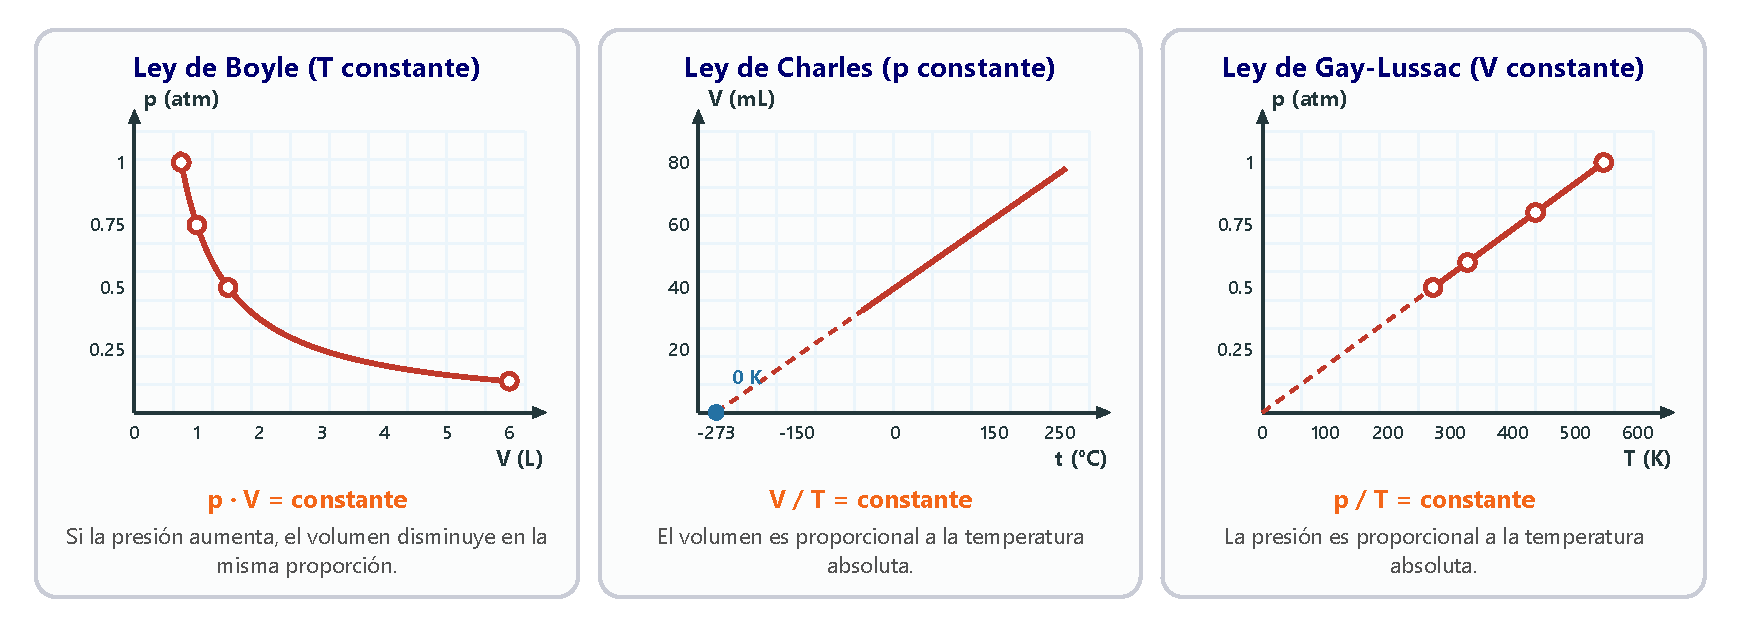
\includegraphics[width=\textwidth]{images/UD5/leyes_gases}
    \caption{Gráficas de las leyes de Boyle, Charles y Gay-Lussac.}
    \label{fig:leyes_gases}
\end{figure}

\subsection{Presión y volumen a temperatura constante: ley de Boyle}

Encerramos un gas en un cilindro con un émbolo móvil y un manómetro, y mantenemos la temperatura constante con un termostato. Al mover el émbolo obtenemos:

\begin{center}
    % --- tabla antigua ---
    % \begin{tblr}{colspec={lcccc}, hlines, vlines, column{1}={bg=ocre!85, fg=white, font=\bfseries}}
        % \(p\) (\unit{\atm}) & \num{1.000} & \num{0.750} & \num{0.500} & \num{0.125} \\
        % \(V\) (\unit{\L}) & \num{0.750} & \num{1.000} & \num{1.500} & \num{6.000} \\
        % \(p \cdot V\) (\unit{\atm\cdot\L}) & \num{0.750} & \num{0.750} & \num{0.750} & \num{0.750} \\
    % \end{tblr}
    % --- tabla nueva ---
    \begin{tabular}{@{}lcccc@{}}
        \toprule
        \textbf{\(p\) (\unit{\atm})} & \num{1.000} & \num{0.750} & \num{0.500} & \num{0.125} \\[3pt]
        \textbf{\(V\) (\unit{\L})} & \num{0.750} & \num{1.000} & \num{1.500} & \num{6.000} \\[3pt]
        \textbf{\(p \cdot V\) (\unit{\atm\cdot\L})} & \num{0.750} & \num{0.750} & \num{0.750} & \num{0.750} \\
        \bottomrule
    \end{tabular}
\end{center}

El producto \(p \cdot V\) es siempre el mismo. Robert Boyle (1662) y, de forma independiente, Edme Mariotte llegaron a esta conclusión:

\begin{definition}[Ley de Boyle-Mariotte]
    A temperatura constante, el volumen de una masa de gas es \textbf{inversamente proporcional} a la presión:
    \[ p \cdot V = \text{constante} \qquad\Rightarrow\qquad p_1 \cdot V_1 = p_2 \cdot V_2 \]
\end{definition}

\begin{example}
    Una bombona de \qty{20}{\L} contiene aire a \qty{12}{\atm}. ¿Qué volumen ocuparía ese aire a \qty{1}{\atm} y a la misma temperatura?

    \textcolor{blue}{Datos:} \(p_1 = \qty{12}{\atm}\); \(V_1 = \qty{20}{\L}\); \(p_2 = \qty{1}{\atm}\).
    \[ p_1 V_1 = p_2 V_2 \;\Rightarrow\; V_2 = \frac{p_1 V_1}{p_2} = \frac{\qty{12}{\atm} \cdot \qty{20}{\L}}{\qty{1}{\atm}} = \textcolor{red}{\qty{240}{\L}} \]
\end{example}

\subsection{Volumen y temperatura a presión constante: ley de Charles}

Si calentamos un gas encerrado en un cilindro con un émbolo que se mueve libremente (la presión no cambia), el gas \textbf{se dilata}, mucho más que los sólidos y los líquidos. Si representamos el volumen frente a la temperatura en grados Celsius obtenemos una recta que, prolongada, corta el eje de temperaturas en \qty{-273}{\celsius}: el \textbf{cero absoluto} (\qty{0}{\kelvin}) (figura~\ref{fig:leyes_gases}).

\begin{definition}[Ley de Charles]
    A presión constante, el volumen de una masa de gas es \textbf{directamente proporcional} a su temperatura absoluta:
    \[ \frac{V}{T} = \text{constante} \qquad\Rightarrow\qquad \frac{V_1}{T_1} = \frac{V_2}{T_2} \]
\end{definition}

\subsection{Presión y temperatura a volumen constante: ley de Gay-Lussac}

Ahora encerramos el gas en un recipiente rígido con un manómetro y lo calentamos al baño María, midiendo la temperatura con un termómetro:

\begin{center}
    % --- tabla antigua ---
    % \begin{tblr}{colspec={cccc}, hlines, vlines, row{1}={bg=ocre!85, fg=white, font=\bfseries}}
        % Experiencia & \(p\) (\unit{\atm}) & \(T\) (\unit{\kelvin}) & \(p/T\) (\unit{\atm\per\kelvin}) \\
        % 1 & \num{0.5} & 273 & \num{1.83e-3} \\
        % 2 & \num{0.6} & 328 & \num{1.83e-3} \\
        % 3 & \num{0.8} & 437 & \num{1.83e-3} \\
        % 4 & \num{1.0} & 546 & \num{1.83e-3} \\
    % \end{tblr}
    % --- tabla nueva ---
    \begin{tabular}{@{}cccc@{}}
        \toprule
        \textbf{Experiencia} & \textbf{\(p\) (\unit{\atm})} & \textbf{\(T\) (\unit{\kelvin})} & \textbf{\(p/T\) (\unit{\atm\per\kelvin})} \\
        \midrule
        1 & \num{0.5} & 273 & \num{1.83e-3} \\[3pt]
        2 & \num{0.6} & 328 & \num{1.83e-3} \\[3pt]
        3 & \num{0.8} & 437 & \num{1.83e-3} \\[3pt]
        4 & \num{1.0} & 546 & \num{1.83e-3} \\
        \bottomrule
    \end{tabular}
\end{center}

\begin{definition}[Ley de Gay-Lussac]
    A volumen constante, la presión de una masa de gas es \textbf{directamente proporcional} a su temperatura absoluta:
    \[ \frac{p}{T} = \text{constante} \qquad\Rightarrow\qquad \frac{p_1}{T_1} = \frac{p_2}{T_2} \]
\end{definition}

\begin{example}
    Un depósito contiene un gas a \qty{2}{\atm} y \qty{15}{\celsius}. Su válvula de seguridad se abre cuando la presión llega a \qty{6}{\atm}. ¿A qué temperatura se abrirá?

    \textcolor{blue}{Datos:} \(p_1 = \qty{2}{\atm}\); \(T_1 = 15 + 273 = \qty{288}{\kelvin}\); \(p_2 = \qty{6}{\atm}\).
    \[ \frac{p_1}{T_1} = \frac{p_2}{T_2} \;\Rightarrow\; T_2 = \frac{p_2 \, T_1}{p_1} = \frac{6 \cdot 288}{2} = \textcolor{red}{\qty{864}{\kelvin}} \;(\qty{591}{\celsius}) \]
\end{example}

\begin{exercise}
    ¿Qué le ocurre a un globo lleno de aire si lo metemos en el frigorífico? ¿Qué ley lo explica?
    \begin{solu}
        Al cabo de un tiempo \textcolor{red}{su volumen disminuye}, porque baja la temperatura del aire de su interior (a presión prácticamente constante). Lo explica la \textcolor{red}{ley de Charles}.
    \end{solu}
\end{exercise}

\begin{exercise}
    ¿Cómo cambia el volumen de un gas a temperatura constante si su presión se reduce a la mitad?
    \begin{solu}
        Como \(p \cdot V\) es constante, si la presión se reduce a la mitad \textcolor{red}{el volumen se duplica}.
    \end{solu}
\end{exercise}

\begin{exercise}
    ¿Cómo cambia el volumen de un gas a presión constante si su temperatura absoluta se triplica? ¿Y si lo que se triplica es su temperatura en grados Celsius?
    \begin{solu}
        Si se triplica la temperatura \textbf{absoluta}, \textcolor{red}{el volumen se triplica} (ley de Charles). Si se triplica la temperatura en \unit{\celsius}, el volumen \textcolor{red}{no} se triplica, porque la ley solo se cumple con temperaturas en kelvin.
    \end{solu}
\end{exercise}

\begin{exercise}
    ¿Qué le ocurre a la presión de un gas encerrado en un recipiente rígido si su temperatura absoluta se reduce a la mitad?
    \begin{solu}
        Según la ley de Gay-Lussac, \textcolor{red}{la presión también se reduce a la mitad}.
    \end{solu}
\end{exercise}

\begin{exercise}
    Un recipiente cerrado contiene un gas a \qty{1.20}{\atm} y \qty{20}{\celsius}.
    \begin{enumerate}[label=\alph*)]
        \item ¿Qué presión habrá si se calienta hasta \qty{50}{\celsius}?
        \item Copia y completa la tabla para otro gas del mismo tipo de experiencia:
        \begin{center}
            % --- tabla antigua ---
            % \begin{tblr}{colspec={lccc}, hlines, vlines, column{1}={bg=ocre!85, fg=white, font=\bfseries}}
                % \(p\) (\unit{\atm}) & \num{1.00} & \ldots & \num{1.50} \\
                % \(T\) (\unit{\kelvin}) & 293 & 373 & \ldots \\
            % \end{tblr}
            % --- tabla nueva ---
            \begin{tabular}{@{}lccc@{}}
                \toprule
                \textbf{\(p\) (\unit{\atm})} & \num{1.00} & \ldots & \num{1.50} \\[3pt]
                \textbf{\(T\) (\unit{\kelvin})} & 293 & 373 & \ldots \\
                \bottomrule
            \end{tabular}
        \end{center}
        \item Representa gráficamente los datos de la tabla.
    \end{enumerate}
    \begin{solu}
        a) \(T_1 = \qty{293}{\kelvin}\); \(T_2 = \qty{323}{\kelvin}\). \(p_2 = p_1 \dfrac{T_2}{T_1} = \num{1.20} \cdot \dfrac{323}{293} = \textcolor{red}{\qty{1.32}{\atm}}\).
        b) \(p = \num{1.00} \cdot \frac{373}{293} = \textcolor{red}{\qty{1.27}{\atm}}\); \(T = 293 \cdot \frac{\num{1.50}}{\num{1.00}} = \textcolor{red}{\qty{439.5}{\kelvin}}\).
        c) Los puntos están sobre una \textcolor{red}{recta que pasa por el origen}, como en la figura~\ref{fig:leyes_gases}.
    \end{solu}
\end{exercise}

\subsection{La ley combinada de los gases ideales}

¿Qué pasa si cambian a la vez la presión, el volumen y la temperatura? Podemos imaginar que el gas pasa del estado inicial (\(p_1\), \(V_1\), \(T_1\)) al final (\(p_2\), \(V_2\), \(T_2\)) en dos etapas (figura~\ref{fig:ley_combinada}):

\begin{enumerate}[label=\numberballblue]
    \item A temperatura constante, la presión pasa de \(p_1\) a \(p_2\) y el volumen de \(V_1\) a un valor intermedio \(V'\). Por la ley de Boyle: \(p_1 V_1 = p_2 V'\).
    \item A presión constante, la temperatura pasa de \(T_1\) a \(T_2\) y el volumen de \(V'\) a \(V_2\). Por la ley de Charles: \(V'/T_1 = V_2/T_2\).
\end{enumerate}

Despejando \(V'\) en las dos expresiones e igualando se obtiene la \textbf{ley combinada de los gases ideales}:

\begin{centeredequation}
    \frac{p_1 \cdot V_1}{T_1} = \frac{p_2 \cdot V_2}{T_2}
\end{centeredequation}

\begin{figure}[H]
    \centering
    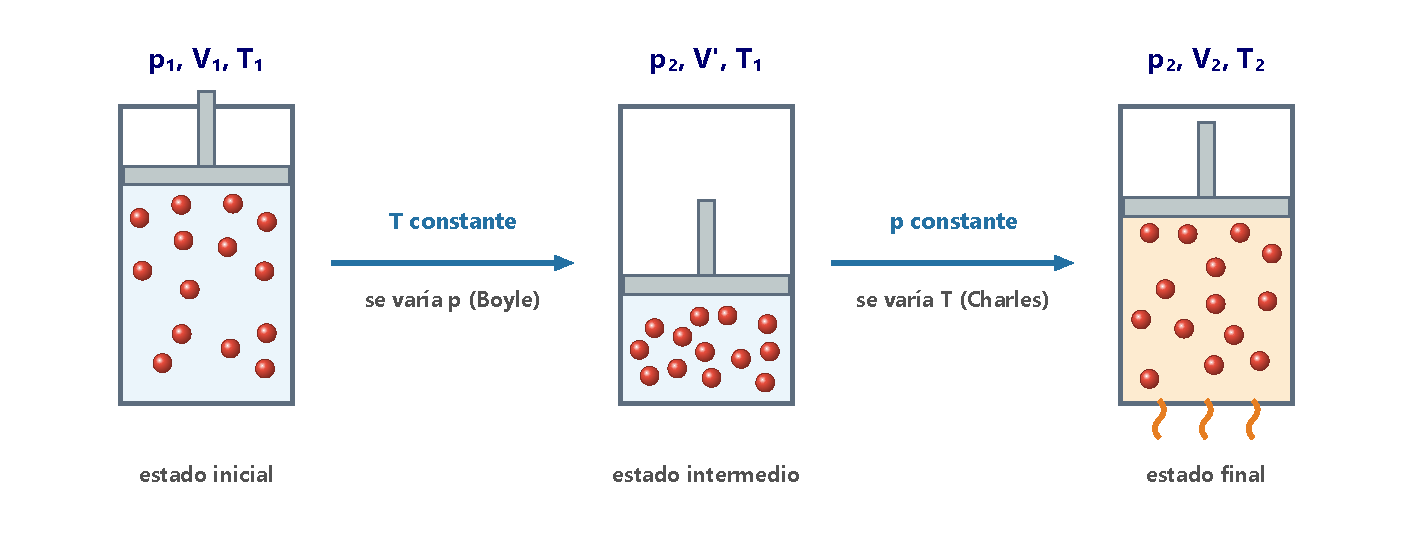
\includegraphics[width=0.85\textwidth]{images/UD5/ley_combinada}
    \caption{Paso de un estado a otro en dos etapas: primero a temperatura constante y después a presión constante.}
    \label{fig:ley_combinada}
\end{figure}

Si la cantidad de gas no cambia, el cociente \(p \cdot V / T\) es constante: si fijamos dos de las tres variables, la tercera queda determinada. Al aplicar la ley hay que tener en cuenta que:
\begin{enumerate}[label=\arabic*.]
    \item A cada lado de la igualdad deben usarse las \textbf{mismas unidades} de presión y de volumen.
    \item La temperatura siempre se expresa en \textbf{kelvin}.
\end{enumerate}

\begin{example}
    Un gas ocupa \qty{12}{\L} a \qty{27}{\celsius} y \qty{1}{\atm}. ¿Qué volumen ocupará a \qty{127}{\celsius} y \qty{2}{\atm}?

    \textcolor{blue}{Datos:} \(V_1 = \qty{12}{\L}\); \(p_1 = \qty{1}{\atm}\); \(T_1 = \qty{300}{\kelvin}\); \(p_2 = \qty{2}{\atm}\); \(T_2 = \qty{400}{\kelvin}\).
    \[ \frac{p_1 V_1}{T_1} = \frac{p_2 V_2}{T_2} \;\Rightarrow\; V_2 = \frac{p_1 V_1 T_2}{T_1 \, p_2} = \frac{1 \cdot 12 \cdot 400}{300 \cdot 2} = \textcolor{red}{\qty{8}{\L}} \]
\end{example}

\begin{exercise}
    Un gas a \qty{20}{\celsius} y \qty{1}{\atm} ocupa \qty{20}{\L}. Si al calentarlo hasta \qty{60}{\celsius} pasa a ocupar \qty{30}{\L}, ¿a qué presión estará?
    \begin{solu}
        \(T_1 = \qty{293}{\kelvin}\); \(T_2 = \qty{333}{\kelvin}\).
        \[ p_2 = \frac{p_1 V_1 T_2}{T_1 V_2} = \frac{1 \cdot 20 \cdot 333}{293 \cdot 30} = \textcolor{red}{\qty{0.76}{\atm}} \]
    \end{solu}
\end{exercise}

\begin{exercise}
    Indica si son verdaderas o falsas estas afirmaciones y corrige las falsas:
    \begin{enumerate}[label=\alph*)]
        \item Según la ley de Boyle, a temperatura constante el volumen de un gas es directamente proporcional a la presión.
        \item A presión constante, el volumen de un gas es directamente proporcional a su temperatura en kelvin.
        \item El cero de la escala Kelvin corresponde a \qty{-273.15}{\celsius}.
    \end{enumerate}
    \begin{solu}
        a) \textcolor{red}{Falsa}: el volumen es \emph{inversamente} proporcional a la presión. b) \textcolor{red}{Verdadera} (ley de Charles). c) \textcolor{red}{Verdadera}.
    \end{solu}
\end{exercise}

\begin{exercise}
    Lee el texto y contesta:

    \begin{quote}
        \emph{La presión de los neumáticos de una moto es esencial: si van demasiado blandos, la rueda se desgasta antes y, en la delantera, la frenada empeora. Un aumento del \qty{10}{\percent} de la temperatura del aire de la rueda aumenta un \qty{10}{\percent} su presión. La presión se suele dar en bar (\(\qty{1}{\atm} = \qty{1.013}{\bar}\)). Se recomienda llevar la rueda delantera a \qty{2.2}{\bar} y la trasera a \qty{2.4}{\bar}, medidas en frío con un manómetro. Si se mide en caliente, hay que sumar \qty{0.3}{\bar} a la presión aconsejada.}
    \end{quote}

    \begin{enumerate}[label=\alph*)]
        \item Expresa en atm y en mmHg las presiones recomendadas.
        \item ¿Por qué es peligroso llevar los neumáticos con menos presión de la indicada?
        \item ¿Qué precauciones hay que tener al medir la presión?
        \item ¿Qué le pasa a la presión del aire si aumenta la temperatura? ¿Qué ley lo explica?
        \item Tras circular una hora, la rueda delantera marca \qty{2.5}{\bar} y la trasera \qty{2.7}{\bar}. ¿Es correcta la presión?
    \end{enumerate}
    \begin{solu}
        a) Delantera: \(\frac{\num{2.2}}{\num{1.013}} = \qty{2.17}{\atm}\); \(\num{2.17} \cdot 760 = \textcolor{red}{\qty{1650}{\mmHg}}\). Trasera: \(\frac{\num{2.4}}{\num{1.013}} = \qty{2.37}{\atm}\); \(\num{2.37} \cdot 760 = \textcolor{red}{\qty{1801}{\mmHg}}\).
        b) Se desgasta antes la banda de rodadura y la frenada es peor.
        c) Medirla en frío o, si se mide en caliente, sumar \qty{0.3}{\bar} a la presión aconsejada.
        d) \textcolor{red}{Aumenta} (ley de Gay-Lussac: el volumen de la rueda es casi constante).
        e) \textcolor{red}{Sí}: en caliente deberían marcar \(\num{2.2} + \num{0.3} = \qty{2.5}{\bar}\) y \(\num{2.4} + \num{0.3} = \qty{2.7}{\bar}\).
    \end{solu}
\end{exercise}

\begin{exercise}
    ¿A qué presión hay que someter \qty{3}{\L} de nitrógeno que están a \qty{1.2}{\atm} para comprimirlos hasta \qty{0.9}{\L} sin cambiar la temperatura? ¿Qué ley has aplicado?
    \begin{solu}
        Ley de \textcolor{red}{Boyle}: \(p_2 = \dfrac{p_1 V_1}{V_2} = \dfrac{\num{1.2} \cdot 3}{\num{0.9}} = \textcolor{red}{\qty{4}{\atm}}\).
    \end{solu}
\end{exercise}

\begin{exercise}
    Tenemos \qty{40}{\cubic\centi\metre} de oxígeno a \qty{760}{\mmHg}. ¿Qué volumen ocupará a \qty{640}{\mmHg} si la temperatura no cambia?
    \begin{solu}
        \(V_2 = \dfrac{p_1 V_1}{p_2} = \dfrac{760 \cdot 40}{640} = \textcolor{red}{\qty{47.5}{\cubic\centi\metre}}\).
    \end{solu}
\end{exercise}

\begin{exercise}
    Un cilindro con un émbolo móvil contiene \qty{30}{\cubic\centi\metre} de gas a \qty{27}{\celsius}. Si el volumen máximo del cilindro es \qty{75}{\cubic\centi\metre}, ¿hasta qué temperatura se puede calentar a presión constante? ¿Qué ley has usado?
    \begin{solu}
        Ley de \textcolor{red}{Charles}, con \(T_1 = \qty{300}{\kelvin}\):
        \(T_2 = T_1 \dfrac{V_2}{V_1} = 300 \cdot \dfrac{75}{30} = \textcolor{red}{\qty{750}{\kelvin}} = \qty{477}{\celsius}\).
    \end{solu}
\end{exercise}

\begin{exercise}
    Un gas ocupa \qty{12}{\cubic\deci\metre} a \qty{0}{\celsius} y \qty{1}{\atm}. ¿Qué volumen ocupará a \qty{50}{\celsius} si la presión no cambia?
    \begin{solu}
        \(V_2 = V_1 \dfrac{T_2}{T_1} = 12 \cdot \dfrac{323}{273} = \textcolor{red}{\qty{14.2}{\cubic\deci\metre}}\).
    \end{solu}
\end{exercise}

\begin{exercise}
    Escribe cómo queda la ley combinada de los gases si a) la presión es constante; b) la temperatura es constante; c) el volumen es constante. ¿Qué nombre recibe cada una?
    \begin{solu}
        a) \(\dfrac{V_1}{T_1} = \dfrac{V_2}{T_2}\): \textcolor{red}{ley de Charles}. b) \(p_1 V_1 = p_2 V_2\): \textcolor{red}{ley de Boyle-Mariotte}. c) \(\dfrac{p_1}{T_1} = \dfrac{p_2}{T_2}\): \textcolor{red}{ley de Gay-Lussac}.
    \end{solu}
\end{exercise}

\begin{exercise}
    Una masa de oxígeno ocupa \qty{25}{\cubic\deci\metre} a \qty{27}{\celsius} y \qty{760}{\mmHg}. ¿Qué volumen ocupará a \qty{87}{\celsius} y \qty{950}{\mmHg}?
    \begin{solu}
        \(T_1 = \qty{300}{\kelvin}\); \(T_2 = \qty{360}{\kelvin}\).
        \[ V_2 = \frac{p_1 V_1 T_2}{T_1 \, p_2} = \frac{760 \cdot 25 \cdot 360}{300 \cdot 950} = \textcolor{red}{\qty{24}{\cubic\deci\metre}} \]
    \end{solu}
\end{exercise}

\begin{exercise}
    Un gas ocupa \qty{3}{\cubic\deci\metre} a \qty{27}{\celsius} y \qty{1}{\atm}. Lo calentamos hasta \qty{54}{\celsius}.
    \begin{enumerate}[label=\alph*)]
        \item Si la presión no cambia, ¿qué volumen ocupará? ¿Se ha duplicado el volumen al duplicar la temperatura en grados Celsius?
        \item Si el volumen no cambia, ¿qué presión tendrá? ¿Se ha duplicado?
    \end{enumerate}
    \begin{solu}
        \(T_1 = \qty{300}{\kelvin}\); \(T_2 = \qty{327}{\kelvin}\).
        a) \(V_2 = 3 \cdot \frac{327}{300} = \textcolor{red}{\qty{3.27}{\cubic\deci\metre}}\). \textcolor{red}{No} se duplica: la proporcionalidad es con la temperatura en kelvin.
        b) \(p_2 = 1 \cdot \frac{327}{300} = \textcolor{red}{\qty{1.09}{\atm}}\). Tampoco se duplica.
    \end{solu}
\end{exercise}

\begin{exercise}
    El aire de los neumáticos de un coche está a \qty{15}{\celsius} y \qty{2.2}{\atm}. Calcula su presión cuando, por el rozamiento con el asfalto, su temperatura llega a \qty{45}{\celsius}.
    \begin{solu}
        \(p_2 = p_1 \dfrac{T_2}{T_1} = \num{2.2} \cdot \dfrac{318}{288} = \textcolor{red}{\qty{2.43}{\atm}}\).
    \end{solu}
\end{exercise}

\begin{exercise}
    Un gas encerrado por un émbolo móvil ocupa \qty{40}{\L} a \qty{27}{\celsius} y \qty{4}{\atm}. ¿Qué volumen ocupará a \qty{1}{\atm} y \qty{0}{\celsius}?
    \begin{solu}
        \(V_2 = \dfrac{p_1 V_1 T_2}{T_1 \, p_2} = \dfrac{4 \cdot 40 \cdot 273}{300 \cdot 1} = \textcolor{red}{\qty{145.6}{\L}}\).
    \end{solu}
\end{exercise}

%========================================================================================
\section{La ley general de los gases. El volumen molar}
%========================================================================================

Según la ley combinada, para una cantidad fija de gas \(p \cdot V / T\) es constante. Si tenemos \textbf{un mol} de gas, esa constante es la misma para todos los gases: es la \textbf{constante universal de los gases}, \(R\). Para \(n\) moles, la constante es \(n \cdot R\), y se obtiene la \textbf{ecuación general de los gases ideales}:

\begin{centeredequation}
    p \cdot V = n \cdot R \cdot T \qquad R = \qty{0.082}{\atm\cdot\L\per\mol\per\kelvin} = \qty{8.31}{\joule\per\mol\per\kelvin}
\end{centeredequation}

Con \(R = \num{0.082}\), la presión debe estar en atmósferas, el volumen en litros y la temperatura en kelvin.

\paragraph{El volumen molar.} Según Avogadro, un mol de cualquier gas ocupa el mismo volumen que un mol de otro gas si se miden a la misma presión y temperatura. Calculemos ese volumen a \qty{0}{\celsius} y \qty{1}{\atm} (condiciones normales):
\[ V = \frac{n R T}{p} = \frac{1 \cdot \num{0.082} \cdot 273}{1} = \qty{22.4}{\L} \]

\begin{definition}[Volumen molar]
    Es el volumen que ocupa un mol de \textbf{cualquier gas} en unas condiciones dadas. A \qty{0}{\celsius} y \qty{1}{\atm} vale \textbf{\qty{22.4}{\L}} y contiene \num{6.022e23} moléculas.
\end{definition}

\begin{remark}
    Actualmente la IUPAC define las \textbf{condiciones estándar} como \qty{273.15}{\kelvin} y \qty{e5}{\pascal} (\qty{0.987}{\atm}); en ellas el volumen molar es \qty{22.7}{\L}. En este curso usaremos el valor clásico de \qty{22.4}{\L}, medido a \qty{0}{\celsius} y \qty{1}{\atm}, al que nos referiremos como «condiciones estándar» (c.\,e.).
\end{remark}

\begin{figure}[H]
    \centering
    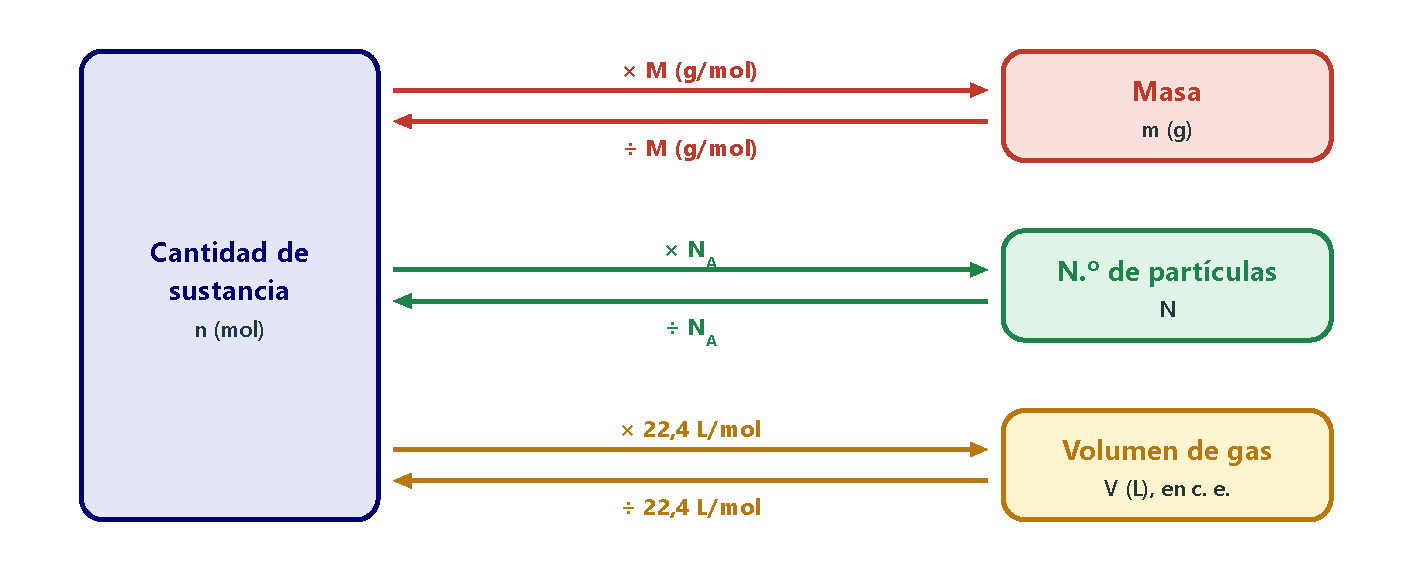
\includegraphics[width=0.85\textwidth]{images/UD5/mol_gas}
    \caption{Relación de la cantidad de sustancia con la masa, el número de partículas y el volumen de un gas en condiciones estándar.}
    \label{fig:mol_gas}
\end{figure}

\begin{example}
    \textbf{¿A qué temperatura están 4 mol de un gas que ocupan \qty{25}{\L} a \qty{4}{\atm}?}
    \[ T = \frac{p V}{n R} = \frac{4 \cdot 25}{4 \cdot \num{0.082}} = \textcolor{red}{\qty{305}{\kelvin}} \]
    \textbf{¿Cuántas moléculas hay en \qty{1}{\cubic\metre} de un gas en condiciones estándar?} \(\qty{1}{\cubic\metre} = \qty{1000}{\L}\):
    \[ n = \frac{\qty{1000}{\L}}{\qty{22.4}{\L\per\mol}} = \qty{44.6}{\mol}; \qquad N = \num{44.6} \cdot \num{6.022e23} = \textcolor{red}{\num{2.69e25}} \text{ moléculas} \]
\end{example}

\begin{exercise}
    ¿Qué volumen ocupan \qty{3}{\mol} de un gas en condiciones estándar?
    \begin{solu}
        \(V = 3 \cdot \num{22.4} = \textcolor{red}{\qty{67.2}{\L}}\).
    \end{solu}
\end{exercise}

\begin{exercise}
    ¿Qué volumen ocupan \num{1.2044e23} moléculas de metano en condiciones estándar?
    \begin{solu}
        \(n = \dfrac{\num{1.2044e23}}{\num{6.022e23}} = \qty{0.2}{\mol}\); \(V = \num{0.2} \cdot \num{22.4} = \textcolor{red}{\qty{4.48}{\L}}\).
    \end{solu}
\end{exercise}

\begin{exercise}
    Completa las frases:
    \begin{enumerate}[label=\alph*)]
        \item El mol, unidad de \ldots, es la cantidad de cualquier conjunto de partículas idénticas que contiene \ldots{} partículas.
        \item Un mol de oxígeno, \ch{O2}, tiene una masa de \ldots{} y ocupa \ldots{} litros en condiciones estándar.
    \end{enumerate}
    \begin{solu}
        a) El mol, unidad de \textcolor{red}{cantidad de sustancia}, contiene \textcolor{red}{\num{6.022e23}} partículas. b) Tiene una masa de \textcolor{red}{\qty{32}{\gram}} y ocupa \textcolor{red}{\qty{22.4}{\L}}.
    \end{solu}
\end{exercise}

\begin{exercise}
    ¿Dónde hay más moléculas: en \qty{5}{\mol} de hidrógeno, \ch{H2}, o en \qty{5}{\mol} de dióxido de carbono, \ch{CO2}? ¿Y más masa?
    \begin{solu}
        Hay el \textcolor{red}{mismo número de moléculas}: \(5 \cdot \num{6.022e23} = \num{3.011e24}\). Tiene más masa el \ch{CO2}: \(5 \cdot 44 = \qty{220}{\gram}\) frente a \(5 \cdot 2 = \qty{10}{\gram}\) de \ch{H2}.
    \end{solu}
\end{exercise}

\begin{exercise}
    Indica si son verdaderas o falsas y corrige las falsas:
    \begin{enumerate}[label=\alph*)]
        \item La ley general de los gases dice que \(p \cdot V / T\) = constante.
        \item El volumen molar es el que ocupa un gas en condiciones estándar.
        \item Un mol de cualquier gas ocupa el mismo volumen que un mol de otro gas si ambos están a la misma presión y temperatura.
        \item \qty{2}{\gram} de hidrógeno ocupan el mismo volumen que \qty{28}{\gram} de nitrógeno aunque no estén en las mismas condiciones.
    \end{enumerate}
    \begin{solu}
        a) \textcolor{red}{Falsa}: la ley general es \(p \cdot V = n \cdot R \cdot T\) (\(pV/T\) = constante es la ley combinada, para una cantidad fija de gas). b) \textcolor{red}{Falsa}: es el volumen que ocupa \emph{un mol} de cualquier gas. c) \textcolor{red}{Verdadera}. d) \textcolor{red}{Falsa}: son \qty{1}{\mol} de cada gas y ocupan el mismo volumen solo si están \emph{en las mismas condiciones}.
    \end{solu}
\end{exercise}

\begin{exercise}
    ¿Cuántas moléculas de nitrógeno hay en \qty{33.6}{\L} de este gas medidos en condiciones estándar?
    \begin{solu}
        \(n = \dfrac{\num{33.6}}{\num{22.4}} = \qty{1.5}{\mol}\); \(N = \num{1.5} \cdot \num{6.022e23} = \textcolor{red}{\num{9.033e23}}\) moléculas.
    \end{solu}
\end{exercise}

\begin{exercise}
    Dos moles de un gas están en un recipiente de \qty{50}{\L} a \qty{27}{\celsius}. a) ¿A qué presión está el gas? b) ¿Cuántas moléculas hay?
    \begin{solu}
        a) \(p = \dfrac{n R T}{V} = \dfrac{2 \cdot \num{0.082} \cdot 300}{50} = \textcolor{red}{\qty{0.98}{\atm}}\). b) \(N = 2 \cdot \num{6.022e23} = \textcolor{red}{\num{1.2044e24}}\) moléculas.
    \end{solu}
\end{exercise}

\begin{exercise}
    Calcula la presión de \qty{0.5}{\mol} de un gas encerrado en un recipiente de \qty{5}{\cubic\deci\metre} a \qty{37}{\celsius}, y el número de moléculas que contiene.
    \begin{solu}
        \(p = \dfrac{\num{0.5} \cdot \num{0.082} \cdot 310}{5} = \textcolor{red}{\qty{2.54}{\atm}}\); \(N = \num{0.5} \cdot \num{6.022e23} = \textcolor{red}{\num{3.011e23}}\) moléculas.
    \end{solu}
\end{exercise}

%========================================================================================
\section{Los sistemas materiales}
%========================================================================================

\begin{definition}[Sistema material]
    Un \textbf{sistema material} es una porción de materia que se separa del resto para estudiarla.
\end{definition}

Según su aspecto, los sistemas materiales se clasifican en (figura~\ref{fig:clasificacion_materia}):
\begin{itemize}
    \item \textbf{Heterogéneos}: no tienen un aspecto uniforme; a simple vista (o con un microscopio) se distinguen sus componentes. Los componentes pueden estar en cualquier proporción y cada uno conserva sus propiedades. Ejemplos: agua y aceite, granito, arena de playa.
    \item \textbf{Homogéneos}: tienen un aspecto uniforme en todos sus puntos. Ejemplos: agua con sal disuelta, agua destilada, aire.
\end{itemize}

\begin{figure}[H]
    \centering
    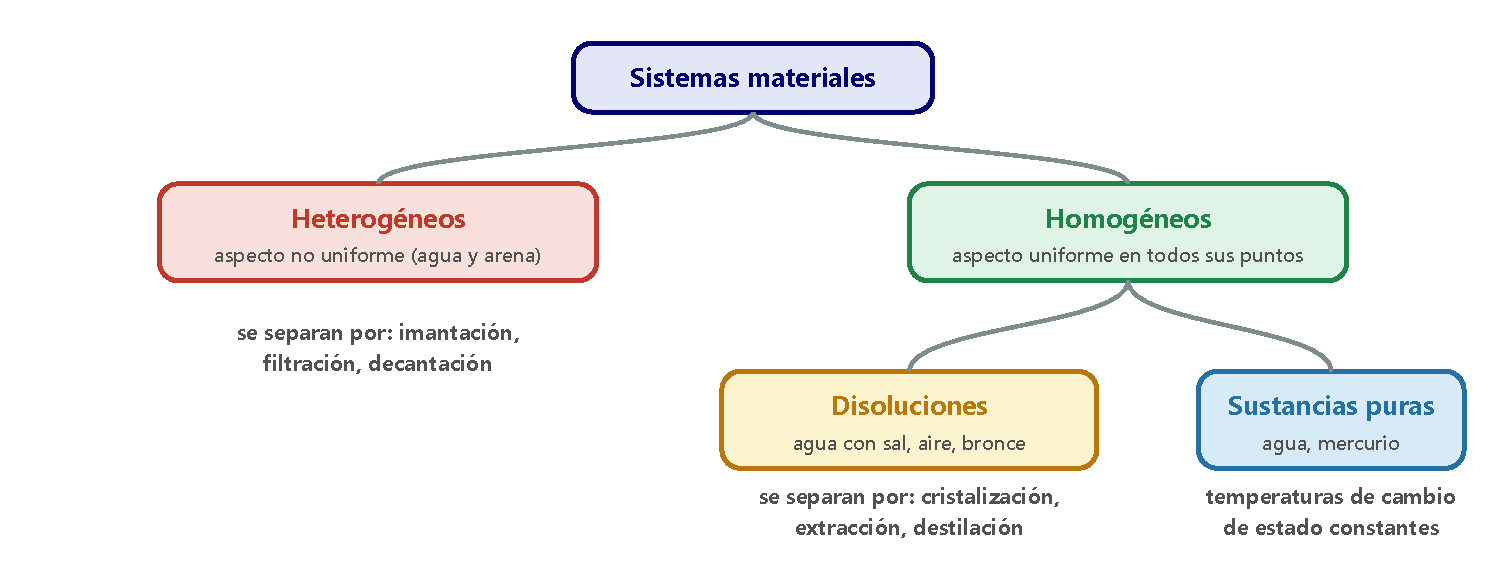
\includegraphics[width=0.95\textwidth]{images/UD5/clasificacion_materia}
    \caption{Clasificación de los sistemas materiales.}
    \label{fig:clasificacion_materia}
\end{figure}

\subsection{¿Cómo se separan los componentes de un sistema heterogéneo?}

Como cada componente conserva sus propiedades, podemos aprovecharlas para separarlos (figura~\ref{fig:separacion_heterogeneos}):
\begin{itemize}
    \item \textbf{Separación magnética.} Separa un sólido magnético (como las limaduras de hierro) de otros que no lo son (arena, sal) acercando un imán.
    \item \textbf{Filtración.} Separa un sólido insoluble de un líquido, por ejemplo arena y agua. Se dobla un papel de filtro, se coloca en un embudo sin que sobresalga y se vierte la mezcla poco a poco ayudándose de una varilla de vidrio. El líquido atraviesa el filtro y el sólido queda retenido.
    \item \textbf{Decantación.} Separa dos líquidos \textbf{inmiscibles} (que no se mezclan) de distinta densidad, como agua y aceite. Se vierte la mezcla en un embudo de decantación y se deja reposar hasta que se formen dos capas. Al abrir la llave sale primero el líquido más denso; cuando ha salido todo, se cierra.
\end{itemize}

\begin{figure}[H]
    \centering
    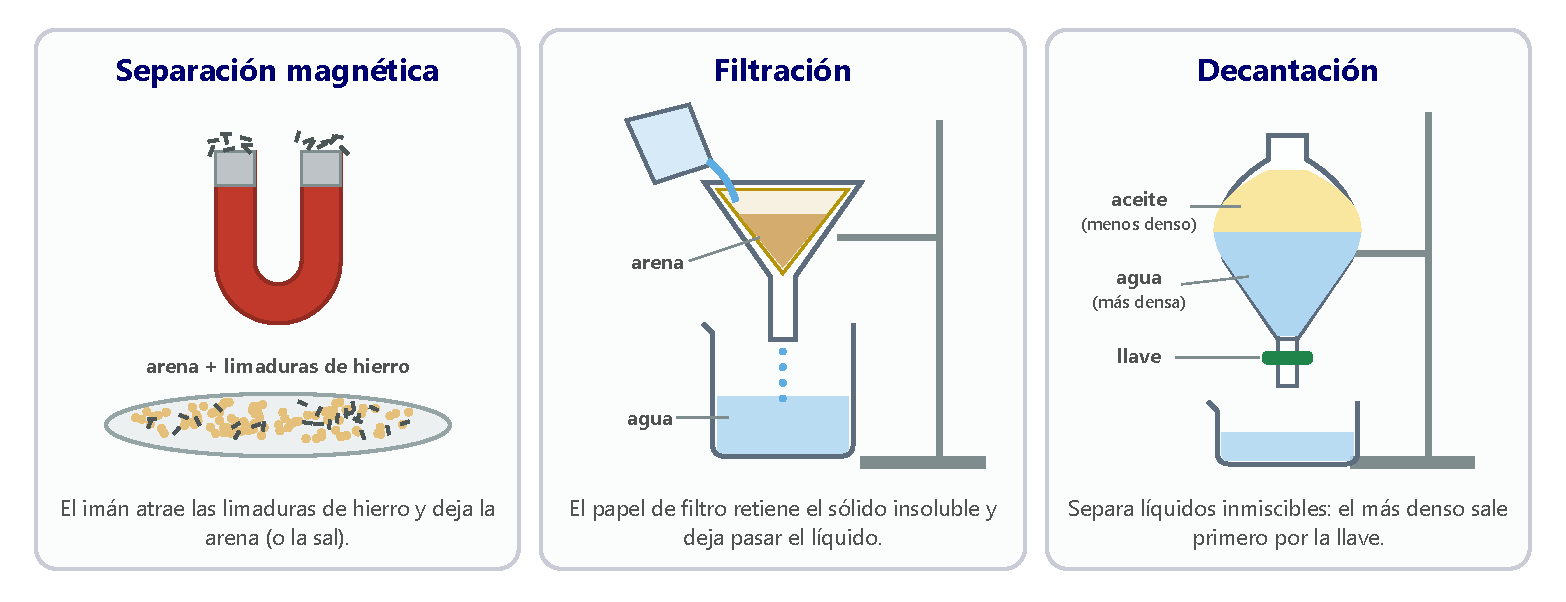
\includegraphics[width=\textwidth]{images/UD5/separacion_heterogeneos}
    \caption{Técnicas para separar los componentes de un sistema heterogéneo.}
    \label{fig:separacion_heterogeneos}
\end{figure}

\begin{exercise}
    Clasifica estos sistemas materiales en homogéneos y heterogéneos: a) agua del grifo; b) agua y arena; c) aceite y vinagre; d) granito; e) aire filtrado; f) vidrio transparente; g) sal común; h) zumo de naranja natural.
    \begin{solu}
        Homogéneos: \textcolor{red}{a), e), f) y g)}. Heterogéneos: \textcolor{red}{b), c), d) y h)} (en el zumo natural se ven la pulpa y otras partículas).
    \end{solu}
\end{exercise}

\begin{exercise}
    ¿Cómo separarías los componentes de estas mezclas?
    \begin{enumerate}[label=\alph*)]
        \item sal y limaduras de hierro;
        \item agua y arena;
        \item limaduras de hierro, arena y agua;
        \item agua y aceite.
    \end{enumerate}
    \begin{solu}
        a) \textcolor{red}{Separación magnética}: el imán atrae el hierro. b) \textcolor{red}{Filtración}: la arena es insoluble en agua. c) Primero \textcolor{red}{filtración} (se separa el agua) y después \textcolor{red}{separación magnética} del hierro y la arena. d) \textcolor{red}{Decantación}: son inmiscibles y tienen distinta densidad.
    \end{solu}
\end{exercise}

\begin{exercise}
    El tetracloruro de carbono es un líquido incoloro, más denso que el agua e inmiscible con ella. ¿Cómo separarías una mezcla de ambos líquidos? ¿Cuál saldrá primero?
    \begin{solu}
        Con un \textcolor{red}{embudo de decantación}, porque son inmiscibles y tienen distinta densidad. Saldrá primero el \textcolor{red}{tetracloruro de carbono}, que es el más denso y queda en la capa inferior.
    \end{solu}
\end{exercise}

%========================================================================================
\section{Sistemas homogéneos: sustancias puras y disoluciones}
%========================================================================================

¿Un sistema homogéneo está formado por una sola sustancia o por varias? Para saberlo se miden sus propiedades características (densidad, temperatura de fusión o de ebullición) y se comprueba si permanecen constantes. Por ejemplo:
\begin{itemize}
    \item El agua con sal empieza a hervir a unos \qty{102}{\celsius}, y su temperatura sigue subiendo mientras hierve.
    \item El agua destilada hierve a \qty{100}{\celsius} y su temperatura no cambia mientras hierve. Lo mismo le pasa al mercurio, pero a \qty{356.7}{\celsius}.
\end{itemize}
El agua destilada y el mercurio son \textbf{sustancias puras}; el agua con sal es una \textbf{disolución}.

\begin{definition}[Sustancia pura y disolución]
    Una \textbf{sustancia pura} tiene una composición fija y unas propiedades características constantes. Una \textbf{disolución} es un sistema material \textbf{homogéneo} y uniforme formado por dos o más sustancias puras en proporción \textbf{variable}.
\end{definition}

\emph{Uniforme} quiere decir que todas las partes de la disolución tienen la misma composición. \emph{Homogéneo} quiere decir que las partículas de los componentes son de tamaño molecular y están repartidas sin ningún orden. En una disolución, las partículas del componente mayoritario, el \textbf{disolvente}, separan y dispersan a las del \textbf{soluto} (figura~\ref{fig:disolucion_particulas}). Así, si dejamos un cristal azul de sulfato de cobre(II) en el fondo de un vaso de agua, poco a poco todo el líquido se vuelve azul: las moléculas de agua chocan con las partículas del cristal y las reparten por todo el vaso.

\begin{figure}[H]
    \centering
    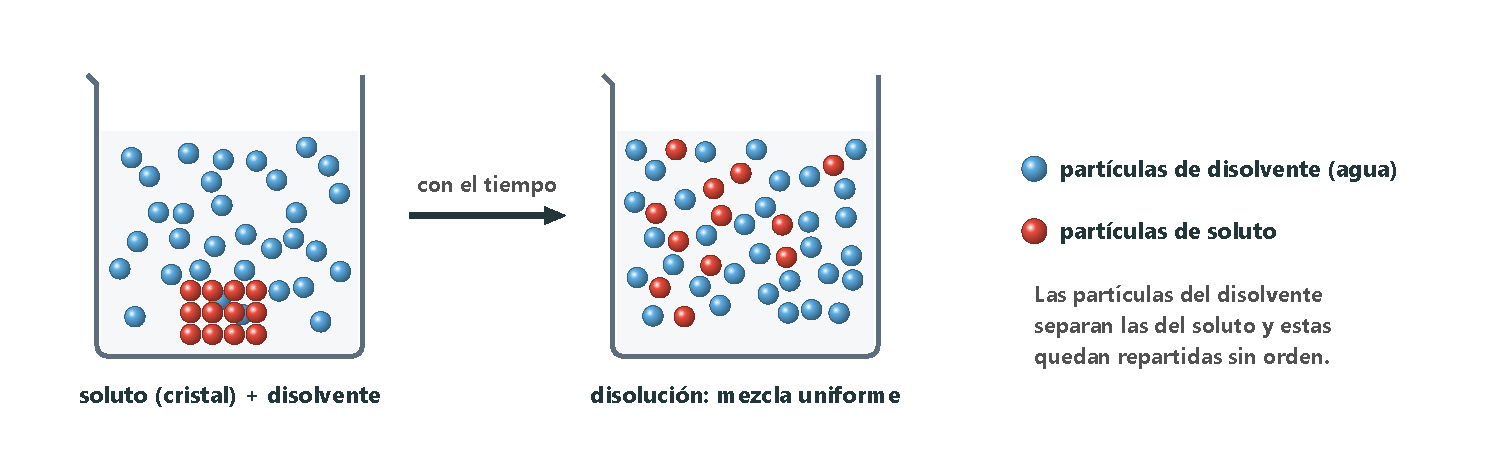
\includegraphics[width=\textwidth]{images/UD5/disolucion_particulas}
    \caption{Al disolverse, las partículas del soluto se reparten entre las del disolvente.}
    \label{fig:disolucion_particulas}
\end{figure}

\begin{exercise}
    Calentamos por separado hasta la ebullición dos líquidos incoloros y transparentes, A y B. Observamos que:
    \begin{enumerate}[label=\arabic*.]
        \item La temperatura de A no cambia mientras hierve y, cuando se evapora todo, no queda nada en el recipiente.
        \item La temperatura de B va subiendo mientras hierve y, cuando se evapora el líquido, queda un residuo blanco.
    \end{enumerate}
    ¿Son sustancias puras o disoluciones?
    \begin{solu}
        A es una \textcolor{red}{sustancia pura}: su temperatura de ebullición es constante y no deja residuo. B es una \textcolor{red}{disolución}: su temperatura de ebullición varía y, al evaporarse el disolvente, queda el soluto sólido.
    \end{solu}
\end{exercise}

\subsection{¿Cómo se expresa la concentración de una disolución?}

\begin{definition}[Concentración]
    La \textbf{concentración} de una disolución es la cantidad de soluto disuelta en una cantidad determinada de disolvente o de disolución.
\end{definition}

\paragraph{Tanto por ciento en masa.} Es la masa de soluto, en gramos, que hay en \qty{100}{\gram} de disolución:
\[ \%\,\text{en masa} = \frac{m_\text{soluto}}{m_\text{disolución}} \cdot 100 \]

\begin{example}
    El oro de 18 quilates es una aleación con un \qty{75}{\percent} en masa de oro; el resto es plata y cobre. ¿Cuánto oro hay en un anillo de \qty{8}{\gram}?
    \[ m_\text{oro} = \frac{75}{100} \cdot \qty{8}{\gram} = \textcolor{red}{\qty{6}{\gram}}; \qquad m_\text{otros metales} = \qty{8}{\gram} - \qty{6}{\gram} = \textcolor{red}{\qty{2}{\gram}} \]
\end{example}

\paragraph{Tanto por ciento en volumen.} Se usa cuando el soluto y el disolvente son líquidos (o gases). Es el volumen de soluto que hay en \qty{100}{\mL} de disolución:
\[ \%\,\text{en volumen} = \frac{V_\text{soluto}}{V_\text{disolución}} \cdot 100 \]

\begin{example}
    ¿Cuánto alcohol hay en un frasco de \qty{250}{\cubic\centi\metre} de alcohol sanitario al \qty{96}{\percent} en volumen?
    \[ V_\text{alcohol} = \frac{96}{100} \cdot \qty{250}{\cubic\centi\metre} = \textcolor{red}{\qty{240}{\cubic\centi\metre}} \]
\end{example}

\paragraph{Concentración en masa.} Es la masa de soluto que hay en cada unidad de volumen de disolución. En el SI se mide en \unit{\kg\per\cubic\metre}, pero lo más habitual es expresarla en \unit{\gram\per\L}:
\[ c = \frac{m_\text{soluto}\,(\unit{\gram})}{V_\text{disolución}\,(\unit{\L})} \]
Por ejemplo, si disolvemos \qty{20}{\gram} de azúcar en agua hasta tener \qty{250}{\mL} de disolución, \(c = \dfrac{\qty{20}{\gram}}{\qty{0.250}{\L}} = \qty{80}{\gram\per\L}\).

\paragraph{Molaridad.}

\begin{definition}[Molaridad, \(M\)]
    La \textbf{molaridad} es la cantidad de soluto, en mol, que hay en un litro de disolución. Se expresa en \unit{\mol\per\L}, unidad que se abrevia como M («molar»):
    \[ M = \frac{n_\text{soluto}\,(\unit{\mol})}{V_\text{disolución}\,(\unit{\L})} \]
\end{definition}

\begin{example}
    Calcula la molaridad de una disolución preparada disolviendo \qty{5.85}{\gram} de cloruro de sodio, \ch{NaCl}, en agua hasta tener \qty{200}{\mL} de disolución (\(A_r\): Na = 23; Cl = \num{35.5}).

    \textcolor{blue}{Masa molar:} \(M(\ch{NaCl}) = \qty{58.5}{\gram\per\mol}\). \quad \textcolor{blue}{Cantidad de soluto:} \(n = \dfrac{\num{5.85}}{\num{58.5}} = \qty{0.1}{\mol}\).
    \[ M = \frac{\qty{0.1}{\mol}}{\qty{0.200}{\L}} = \textcolor{red}{\qty{0.5}{\mol\per\L}} \;(\num{0.5}\,\text{M}) \]
\end{example}

\begin{exercise}
    El acero inoxidable de algunos cuchillos tiene un \qty{0.3}{\percent} de carbono, un \qty{18}{\percent} de cromo y un \qty{8}{\percent} de níquel (el resto es hierro). ¿Qué masa de cada elemento hay en una hoja de \qty{200}{\gram}?
    \begin{solu}
        C: \(\frac{\num{0.3}}{100} \cdot 200 = \textcolor{red}{\qty{0.6}{\gram}}\); Cr: \(\frac{18}{100} \cdot 200 = \textcolor{red}{\qty{36}{\gram}}\); Ni: \(\frac{8}{100} \cdot 200 = \textcolor{red}{\qty{16}{\gram}}\); Fe: \(200 - \num{52.6} = \textcolor{red}{\qty{147.4}{\gram}}\).
    \end{solu}
\end{exercise}

\begin{exercise}
    Un joyero funde \qty{15}{\gram} de oro con \qty{5}{\gram} de plata. ¿Cuál es el tanto por ciento en masa de cada metal en la aleación?
    \begin{solu}
        \(m_\text{aleación} = 15 + 5 = \qty{20}{\gram}\). \(\%\,\text{oro} = \frac{15}{20} \cdot 100 = \textcolor{red}{\qty{75}{\percent}}\); \(\%\,\text{plata} = \frac{5}{20} \cdot 100 = \textcolor{red}{\qty{25}{\percent}}\).
    \end{solu}
\end{exercise}

\begin{exercise}
    ¿Qué volumen de un líquido debes usar para preparar \qty{500}{\cubic\centi\metre} de una disolución acuosa al \qty{70}{\percent} en volumen?
    \begin{solu}
        \(V = \frac{70}{100} \cdot 500 = \textcolor{red}{\qty{350}{\cubic\centi\metre}}\), completando con agua hasta \qty{500}{\cubic\centi\metre}.
    \end{solu}
\end{exercise}

\begin{exercise}
    Calcula la molaridad de una disolución que contiene \qty{12}{\gram} de hidróxido de sodio, \ch{NaOH}, en \qty{1}{\L} de disolución (\(A_r\): Na = 23; O = 16; H = 1).
    \begin{solu}
        \(M(\ch{NaOH}) = \qty{40}{\gram\per\mol}\); \(n = \frac{12}{40} = \qty{0.3}{\mol}\); \(M = \frac{\num{0.3}}{1} = \textcolor{red}{\qty{0.3}{\mol\per\L}}\).
    \end{solu}
\end{exercise}

\begin{exercise}
    ¿Qué masa de \ch{NaOH} hay que disolver para preparar \qty{250}{\mL} de disolución \num{0.2} M?
    \begin{solu}
        \(n = M \cdot V = \num{0.2} \cdot \num{0.250} = \qty{0.05}{\mol}\); \(m = \num{0.05} \cdot 40 = \textcolor{red}{\qty{2}{\gram}}\).
    \end{solu}
\end{exercise}

\begin{exercise}
    Se disuelven \qty{20}{\gram} de bromuro de potasio, \ch{KBr}, en agua hasta tener \qty{400}{\mL} de disolución. Calcula su molaridad (\(A_r\): K = 39; Br = 80).
    \begin{solu}
        \(M(\ch{KBr}) = \qty{119}{\gram\per\mol}\); \(n = \frac{20}{119} = \qty{0.168}{\mol}\); \(M = \frac{\num{0.168}}{\num{0.400}} = \textcolor{red}{\qty{0.42}{\mol\per\L}}\).
    \end{solu}
\end{exercise}

\begin{exercise}
    Se prepara una disolución con \qty{1}{\gram} de cloruro de potasio y \qty{2}{\gram} de cloruro de sodio en \qty{500}{\gram} de agua. ¿Cuál es el tanto por ciento en masa de cada componente?
    \begin{solu}
        \(m_\text{disolución} = 1 + 2 + 500 = \qty{503}{\gram}\).
        \(\%\,\ch{KCl} = \frac{1}{503} \cdot 100 = \textcolor{red}{\qty{0.199}{\percent}}\); \(\%\,\ch{NaCl} = \frac{2}{503} \cdot 100 = \textcolor{red}{\qty{0.398}{\percent}}\); \(\%\,\text{agua} = \frac{500}{503} \cdot 100 = \textcolor{red}{\qty{99.40}{\percent}}\).
    \end{solu}
\end{exercise}

\begin{exercise}
    Para fabricar una joya de \qty{12}{\gram}, un joyero usa una aleación con un \qty{80}{\percent} de oro y un \qty{20}{\percent} de níquel. ¿Qué masa de cada metal necesita?
    \begin{solu}
        Oro: \(\frac{80}{100} \cdot 12 = \textcolor{red}{\qty{9.6}{\gram}}\); níquel: \(\frac{20}{100} \cdot 12 = \textcolor{red}{\qty{2.4}{\gram}}\).
    \end{solu}
\end{exercise}

\begin{exercise}
    Un bronce contiene un \qty{90}{\percent} de cobre y un \qty{10}{\percent} de estaño. ¿Qué masa de cada metal hay que fundir para fabricar una campana de \qty{25}{\kg}?
    \begin{solu}
        Cobre: \(\frac{90}{100} \cdot 25 = \textcolor{red}{\qty{22.5}{\kg}}\); estaño: \(\frac{10}{100} \cdot 25 = \textcolor{red}{\qty{2.5}{\kg}}\).
    \end{solu}
\end{exercise}

\begin{exercise}
    Un latón tiene un \qty{65}{\percent} de cobre y un \qty{35}{\percent} de zinc. ¿Qué masa de cada metal hace falta para una plancha de latón de \qty{40}{\kg}?
    \begin{solu}
        Cobre: \(\frac{65}{100} \cdot 40 = \textcolor{red}{\qty{26}{\kg}}\); zinc: \(\frac{35}{100} \cdot 40 = \textcolor{red}{\qty{14}{\kg}}\).
    \end{solu}
\end{exercise}

\begin{exercise}
    En el envase de un colutorio de \qty{250}{\mL} pone: «Composición: \qty{0.12}{\percent} de digluconato de clorhexidina y \qty{2}{\percent} de xilitol» (gramos por cada \qty{100}{\mL}).
    \begin{enumerate}[label=\alph*)]
        \item ¿Qué cantidad de cada sustancia hay en el frasco?
        \item Cada enjuague se hace con \qty{15}{\mL}. ¿Qué cantidad de cada componente se usa en un enjuague?
    \end{enumerate}
    \begin{solu}
        a) Clorhexidina: \(\frac{\num{0.12}}{100} \cdot 250 = \textcolor{red}{\qty{0.3}{\gram}}\); xilitol: \(\frac{2}{100} \cdot 250 = \textcolor{red}{\qty{5}{\gram}}\).
        b) Clorhexidina: \(\frac{\num{0.12}}{100} \cdot 15 = \textcolor{red}{\qty{0.018}{\gram}}\); xilitol: \(\frac{2}{100} \cdot 15 = \textcolor{red}{\qty{0.3}{\gram}}\).
    \end{solu}
\end{exercise}

\begin{exercise}
    El prospecto de un jarabe dice: «Solución oral: \qty{150}{\mL}. Composición: \qty{4}{\milli\gram\per\mL} de principio activo. Tomar \qty{5}{\mL} cada ocho horas».
    \begin{enumerate}[label=\alph*)]
        \item ¿Cuánto principio activo hay en el frasco?
        \item ¿Cuánto se toma en cada dosis?
        \item ¿Y en un día?
    \end{enumerate}
    \begin{solu}
        a) \(4 \cdot 150 = \textcolor{red}{\qty{600}{\milli\gram}}\). b) \(4 \cdot 5 = \textcolor{red}{\qty{20}{\milli\gram}}\). c) Tres dosis: \(\textcolor{red}{\qty{60}{\milli\gram}}\).
    \end{solu}
\end{exercise}

\begin{exercise}
    Una disolución de \ch{HCl} contiene \qty{7.3}{\gram} de soluto en \qty{250}{\cubic\centi\metre} de disolución. Calcula su molaridad (\(A_r\): Cl = \num{35.5}; H = 1).
    \begin{solu}
        \(M(\ch{HCl}) = \qty{36.5}{\gram\per\mol}\); \(n = \frac{\num{7.3}}{\num{36.5}} = \qty{0.2}{\mol}\); \(M = \frac{\num{0.2}}{\num{0.250}} = \textcolor{red}{\qty{0.8}{\mol\per\L}}\).
    \end{solu}
\end{exercise}

\begin{exercise}
    Se disuelven \qty{17.1}{\gram} de sacarosa (azúcar, \(M = \qty{342}{\gram\per\mol}\)) en agua hasta \qty{500}{\mL} de disolución. ¿Cuál es su molaridad?
    \begin{solu}
        \(n = \frac{\num{17.1}}{342} = \qty{0.05}{\mol}\); \(M = \frac{\num{0.05}}{\num{0.500}} = \textcolor{red}{\qty{0.1}{\mol\per\L}}\).
    \end{solu}
\end{exercise}

\begin{exercise}
    Una disolución contiene \qty{49}{\gram} de ácido sulfúrico, \ch{H2SO4}, en \qty{2}{\L}. ¿Cuál es su molaridad? (\(A_r\): S = 32).
    \begin{solu}
        \(M(\ch{H2SO4}) = 2 + 32 + 64 = \qty{98}{\gram\per\mol}\); \(n = \frac{49}{98} = \qty{0.5}{\mol}\); \(M = \frac{\num{0.5}}{2} = \textcolor{red}{\qty{0.25}{\mol\per\L}}\).
    \end{solu}
\end{exercise}

\begin{exercise}
    Calcula la molaridad de una disolución preparada disolviendo \qty{29.25}{\gram} de \ch{NaCl} en agua hasta tener \qty{250}{\mL} de disolución.
    \begin{solu}
        \(n = \frac{\num{29.25}}{\num{58.5}} = \qty{0.5}{\mol}\); \(M = \frac{\num{0.5}}{\num{0.250}} = \textcolor{red}{\qty{2}{\mol\per\L}}\).
    \end{solu}
\end{exercise}

\begin{exercise}
    Asigna a cada frasco su etiqueta: \num{0.1} M, \num{0.5} M, 1 M o 2 M.
    \begin{enumerate}[label=\alph*)]
        \item \qty{20}{\gram} de \ch{NaOH} en \qty{1}{\L};
        \item \qty{80}{\gram} de \ch{NaOH} en \qty{1}{\L};
        \item \qty{4}{\gram} de \ch{NaOH} en \qty{100}{\mL};
        \item \qty{0.4}{\gram} de \ch{NaOH} en \qty{100}{\mL}.
    \end{enumerate}
    \begin{solu}
        \textcolor{blue}{\(M(\ch{NaOH}) = \qty{40}{\gram\per\mol}\).} a) \(\frac{\num{0.5}}{1}\) \(\Rightarrow\) \textcolor{red}{\num{0.5} M}. b) \(\frac{2}{1}\) \(\Rightarrow\) \textcolor{red}{2 M}. c) \(\frac{\num{0.1}}{\num{0.1}}\) \(\Rightarrow\) \textcolor{red}{1 M}. d) \(\frac{\num{0.01}}{\num{0.1}}\) \(\Rightarrow\) \textcolor{red}{\num{0.1} M}.
    \end{solu}
\end{exercise}

\begin{exercise}
    Indica la molaridad de una disolución que contiene \qty{11.2}{\gram} de hidróxido de potasio, \ch{KOH}, en \qty{2}{\L} de disolución (\(A_r\): K = 39).
    \begin{solu}
        \(M(\ch{KOH}) = \qty{56}{\gram\per\mol}\); \(n = \frac{\num{11.2}}{56} = \qty{0.2}{\mol}\); \(M = \frac{\num{0.2}}{2} = \textcolor{red}{\qty{0.1}{\mol\per\L}}\).
    \end{solu}
\end{exercise}

\subsection{¿Cómo se prepara una disolución de concentración conocida?}

Queremos preparar \qty{250}{\mL} de disolución 1 M de cloruro de sodio. Primero calculamos la masa de soluto:
\[ n = M \cdot V = \qty{1}{\mol\per\L} \cdot \qty{0.250}{\L} = \qty{0.25}{\mol}; \qquad m = n \cdot M(\ch{NaCl}) = \num{0.25} \cdot \num{58.5} = \qty{14.625}{\gram} \]
Después seguimos estos pasos (figura~\ref{fig:preparar_disolucion}):

\begin{enumerate}[label=\numberballgreen]
    \item Pesamos \qty{14.63}{\gram} de \ch{NaCl} en un vaso de precipitados con una balanza digital.
    \item Añadimos unos \qty{100}{\mL} de agua destilada y disolvemos la sal con una varilla de vidrio.
    \item Trasvasamos la disolución a un matraz aforado de \qty{250}{\mL} con ayuda de la varilla y de un embudo. Enjuagamos el vaso con un poco de agua y la echamos también al matraz.
    \item Añadimos agua destilada poco a poco hasta \textbf{enrasar}: la parte baja del menisco debe tocar la marca del aforo.
\end{enumerate}

\begin{figure}[H]
    \centering
    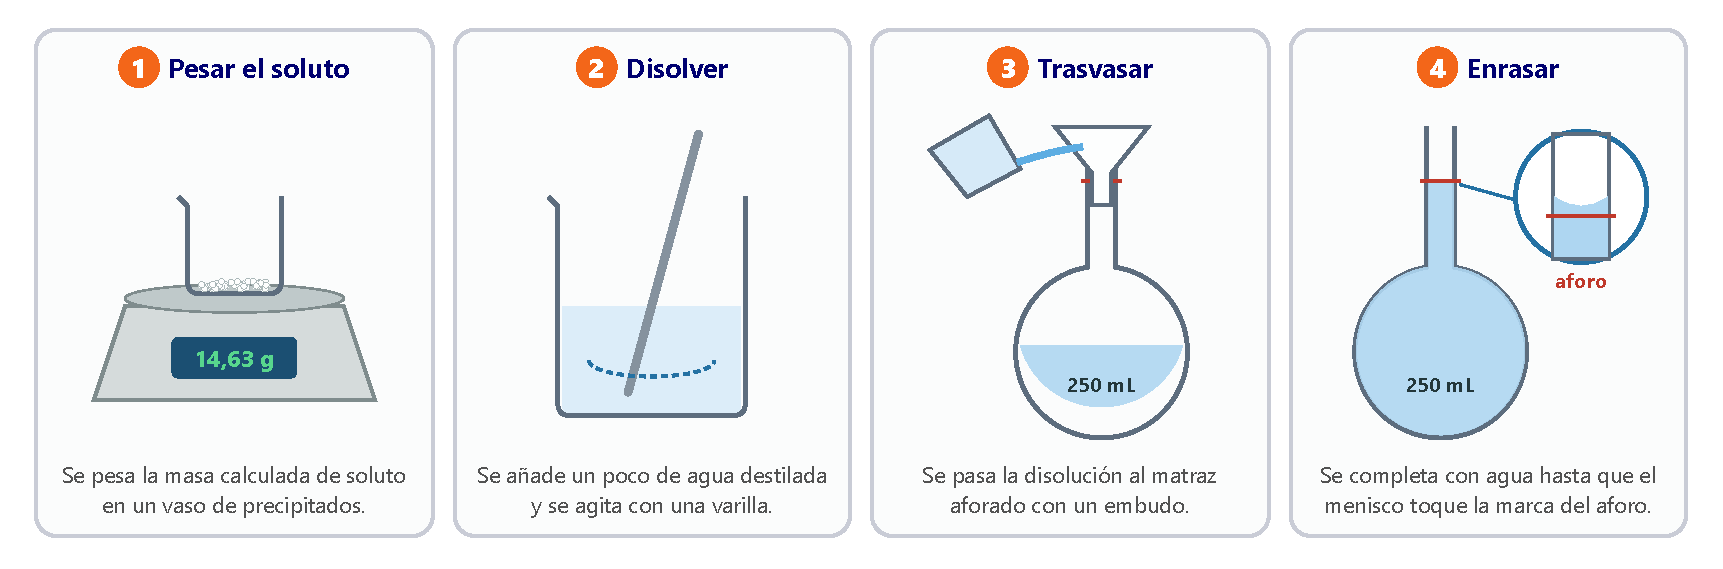
\includegraphics[width=\textwidth]{images/UD5/preparar_disolucion}
    \caption{Pasos para preparar una disolución de concentración conocida.}
    \label{fig:preparar_disolucion}
\end{figure}

\begin{exercise}
    Explica con detalle cómo prepararías \qty{250}{\mL} de disolución \num{0.2} M de cloruro de potasio, \ch{KCl} (\(A_r\): K = 39; Cl = \num{35.5}). ¿Qué material de laboratorio necesitas?
    \begin{solu}
        \textcolor{blue}{Cálculo:} \(n = \num{0.2} \cdot \num{0.250} = \qty{0.05}{\mol}\); \(m = \num{0.05} \cdot \num{74.5} = \textcolor{red}{\qty{3.725}{\gram}}\) de \ch{KCl}.
        \textcolor{blue}{Procedimiento:} se pesan \qty{3.73}{\gram} de \ch{KCl} en un vaso de precipitados con una balanza; se añade un poco de agua destilada y se disuelve con una varilla; se trasvasa a un matraz aforado de \qty{250}{\mL} con un embudo; se añade agua destilada hasta enrasar.
        \textcolor{blue}{Material:} balanza, vaso de precipitados, varilla de vidrio, embudo, matraz aforado de \qty{250}{\mL}, frasco lavador con agua destilada.
    \end{solu}
\end{exercise}

\begin{exercise}
    ¿Qué masa de cloruro de sodio necesitas para preparar \qty{500}{\mL} de disolución acuosa \num{0.2} M?
    \begin{solu}
        \(n = \num{0.2} \cdot \num{0.500} = \qty{0.1}{\mol}\); \(m = \num{0.1} \cdot \num{58.5} = \textcolor{red}{\qty{5.85}{\gram}}\) de \ch{NaCl}, que se disuelven en agua hasta completar \qty{500}{\mL} en un matraz aforado.
    \end{solu}
\end{exercise}

\subsection{¿Cómo se separan los componentes de una disolución?}

\begin{itemize}
    \item \textbf{Cristalización.} Separa un \textbf{soluto sólido} del disolvente; es el proceso inverso a la disolución. Se calienta la disolución para evaporar parte del disolvente, se filtra para eliminar impurezas y se deja enfriar en un cristalizador. Si el enfriamiento es lento, se forman cristales grandes; si es rápido, pequeños.
    \item \textbf{Extracción con disolventes.} Aprovecha que una sustancia es más soluble en un disolvente que en otro. Por ejemplo, el bromo es más soluble en tetracloruro de carbono que en agua. Si añadimos \ch{CCl4} (inmiscible con el agua) a una disolución de bromo en agua y agitamos, el bromo pasa al \ch{CCl4}. Después se separan las dos capas con un embudo de decantación.
    \item \textbf{Destilación simple.} Separa dos líquidos con \textbf{distinta temperatura de ebullición}. Al calentar la disolución en un matraz, el líquido más volátil se evapora antes; su vapor pasa por un \textbf{refrigerante}, por el que circula agua fría, se condensa y se recoge en un vaso o un Erlenmeyer. En el matraz queda el otro componente.
\end{itemize}

\begin{figure}[H]
    \centering
    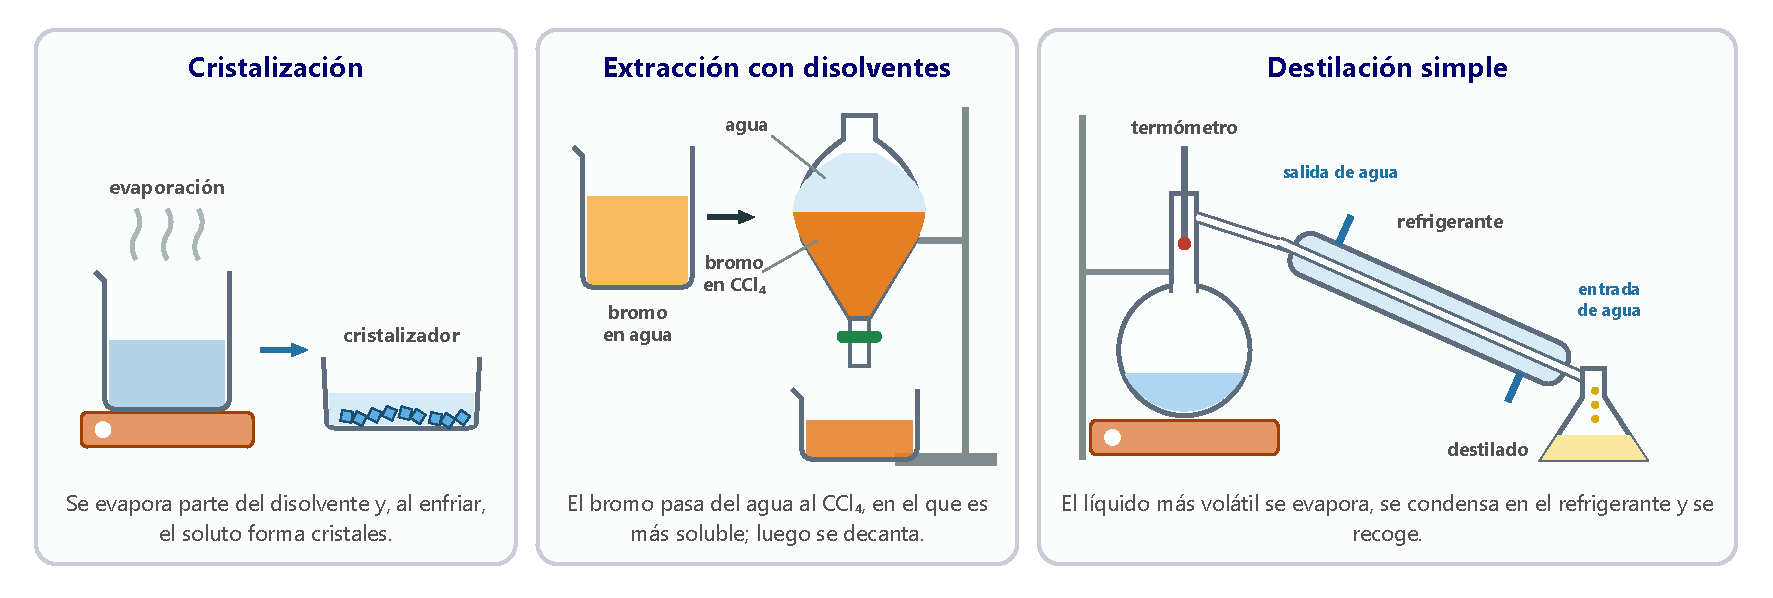
\includegraphics[width=\textwidth]{images/UD5/separacion_disoluciones}
    \caption{Técnicas para separar los componentes de una disolución.}
    \label{fig:separacion_disoluciones}
\end{figure}

\begin{exercise}
    ¿Cuándo se puede usar la extracción con disolventes para separar los componentes de una disolución? Describe el procedimiento.
    \begin{solu}
        Cuando hay un segundo disolvente, \textcolor{red}{inmiscible con el primero}, en el que el soluto es \textcolor{red}{mucho más soluble}. Se añade ese disolvente, se agita para que el soluto pase a él, se deja reposar hasta que se formen dos capas y se separan con un embudo de decantación. Por ejemplo, las grasas son insolubles en agua pero solubles en tolueno.
    \end{solu}
\end{exercise}

\begin{exercise}
    ¿Cuándo se puede usar la cristalización? ¿Sirve para separar los componentes de una disolución en la que el soluto y el disolvente son líquidos?
    \begin{solu}
        Cuando el soluto es un \textcolor{red}{sólido} disuelto en un líquido que se puede evaporar. \textcolor{red}{No} sirve si los dos componentes son líquidos: en ese caso se usa la destilación.
    \end{solu}
\end{exercise}

\begin{exercise}
    ¿Cuándo se puede usar la destilación para separar dos líquidos? ¿Podría usarse para recuperar el agua de una disolución de sal?
    \begin{solu}
        Cuando los dos líquidos tienen \textcolor{red}{distintas temperaturas de ebullición}. \textcolor{red}{Sí}: el agua se evapora, se condensa en el refrigerante y se recoge, y la sal queda en el matraz.
    \end{solu}
\end{exercise}

\begin{exercise}
    ¿En qué técnica (cristalización, extracción con disolventes o destilación) usarías cada uno de estos materiales? Un material puede servir para más de una.
    \begin{enumerate}[label=\alph*)]
        \item placa calefactora;
        \item embudo;
        \item embudo de decantación;
        \item cristalizador;
        \item matraz de destilación;
        \item refrigerante.
    \end{enumerate}
    \begin{solu}
        a) \textcolor{red}{Cristalización y destilación}. b) \textcolor{red}{Cristalización} (para filtrar). c) \textcolor{red}{Extracción}. d) \textcolor{red}{Cristalización}. e) y f) \textcolor{red}{Destilación}.
    \end{solu}
\end{exercise}

\begin{exercise}
    Describe cómo separarías los componentes de: a) una disolución de sulfato de cobre(II) en agua; b) una disolución de yodo en agua; c) una mezcla de alcohol y agua.
    \begin{solu}
        a) \textcolor{red}{Cristalización}: se evapora parte del agua y, al enfriar, cristaliza el sulfato de cobre(II). b) \textcolor{red}{Extracción con disolventes}: se añade un disolvente inmiscible con el agua en el que el yodo es más soluble (por ejemplo, \ch{CCl4}) y después se decanta. c) \textcolor{red}{Destilación simple}: el alcohol hierve a menor temperatura (\qty{78}{\celsius}) que el agua.
    \end{solu}
\end{exercise}
